%% ============================================================
%%  Deferred Asynchronous Post-Quantum Signature Verification
%%  for Low-Latency TLS 1.3 Handshakes
%%  Revised manuscript (addresses Computer Networks reviews of
%%  COMNET-D-25-04940R2, Reviewers #4 and #5)
%%
%%  IMPORTANT: every \authorinput{...} marker (printed in red)
%%  flags information or data that only the authors can supply.
%%  Do NOT submit until every marker has been resolved.
%%  See AUTHOR_ACTION_ITEMS.md.
%% ============================================================
\documentclass[preprint,10pt,3p]{elsarticle}

%% ---- Core packages -----------------------------------------
\usepackage[T1]{fontenc}
\usepackage[utf8]{inputenc}
\usepackage{lmodern}
\usepackage{amsmath,amssymb}
\usepackage{graphicx}
\usepackage{booktabs}
\usepackage{multirow}
\usepackage{array}
\usepackage{xcolor}
\usepackage{url}
\usepackage[protrusion=true,expansion=false]{microtype}
\usepackage{enumitem}
\usepackage[ruled,vlined,linesnumbered]{algorithm2e}
\usepackage{tikz}
\usetikzlibrary{arrows.meta,positioning,calc,decorations.pathreplacing}
\usepackage{geometry}
\geometry{margin=1.8cm, top=2cm, bottom=2cm}
\usepackage[hidelinks]{hyperref}

%% ---- Float placement tuning --------------------------------
\renewcommand{\topfraction}{0.90}
\renewcommand{\bottomfraction}{0.90}
\renewcommand{\textfraction}{0.07}
\renewcommand{\floatpagefraction}{0.85}

\graphicspath{{figures/}}

%% ---- Convenience macros ------------------------------------
\newcommand{\Dt}{\ensuremath{\Delta t}}
\newcommand{\ms}{\,ms}
\newcommand{\state}[1]{\textsc{#1}}
%% Marks information that must be supplied by the authors before submission.
\newcommand{\authorinput}[1]{\textcolor{red}{\textbf{[AUTHOR INPUT: #1]}}}

\journal{\authorinput{target journal}}

%% ============================================================
\begin{document}
\begin{frontmatter}

\title{Deferred Asynchronous Post-Quantum Signature Verification for
Low-Latency TLS~1.3 Handshakes}

\author[au1]{Tahera Begum Abdul\corref{cor1}}
\ead{taherabegum.abdul@gmail.com}
\author[au1]{K.~Venkata Ramana}
\cortext[cor1]{Corresponding author}
\address[au1]{Department of Computer Science and Systems Engineering,
Andhra University, Visakhapatnam, Andhra Pradesh, India}

%% ---- Abstract ----------------------------------------------
\begin{abstract}
Migrating TLS~1.3 server authentication to post-quantum (PQ) signatures is
urgent not because recorded traffic can be decrypted later---that threat is
addressed by hybrid key exchange---but because public-key infrastructures
take many years to migrate and must be quantum-safe \emph{before} a
cryptographically relevant quantum computer can forge classical signatures
in real time.  During the transition, many deployments are expected to use
hybrid authentication, in which a classical (ECDSA) and a PQ (ML-DSA or
FN-DSA) signature must both verify.  This paper studies one component of
the resulting handshake cost: the client-side verification of the PQ
signature component.

We present \textit{Deferred Asynchronous PQ Verification} (DAPV), a
client-side, implementation-level change to the TLS~1.3 handshake state
machine that requires no change to the wire format or to the server.  The
classical component is verified synchronously and the handshake completes
in a \state{provisional} state; the PQ component, already bound into the
handshake transcript, is verified by a background worker, after which the
session is promoted to \state{fully\_authenticated} or terminated.  We
specify the semantics of the provisional state (permitted data, session
tickets, alerts, and an application-facing API), implement a proof of
concept in OpenSSL~3.2 with the Open Quantum Safe provider, and evaluate it
for P-256\,+\,ML-DSA-44 and P-256\,+\,FN-DSA-512.  In our single-host
testbed DAPV lowers client-observed handshake latency by an RTT-independent
offset of about 14--21\ms\ and raises the completed-handshake rate by
31--36\%.  We show, however, that the arithmetic of PQ verification costs
below 0.15\ms, so the measured gain is attributable to non-arithmetic costs
of the synchronous verification path of the prototype rather than to the
cryptography itself; we discuss what this implies for when deferral is
worthwhile (long certificate chains, multi-algorithm hybrids, slower schemes
and constrained devices).  Finally, we bound the data that can be exposed
during the provisional window, identify a denial-of-service vector specific
to deferred verification, and give mitigations.
\end{abstract}

\begin{keyword}
Post-quantum cryptography \sep TLS~1.3 \sep Hybrid authentication \sep
Deferred verification \sep ML-DSA \sep FN-DSA \sep Handshake latency
\end{keyword}
\end{frontmatter}

%% ============================================================
\section{Introduction}
\label{sec:intro}

\subsection{Why post-quantum authentication, and why now}

The public-key algorithms used by TLS today---ECDH/X25519 for key exchange
and RSA or ECDSA for authentication---rely on the hardness of integer
factorisation and discrete logarithms, both of which are solved efficiently
by Shor's algorithm~\cite{Shor1994} on a sufficiently large quantum
computer.  The two uses of public-key cryptography in TLS, however, face
quantum threats of a different nature and urgency.

\emph{Confidentiality} is threatened today by the ``harvest now, decrypt
later'' (HNDL) strategy~\cite{Alnahawi2024}: an adversary records encrypted
sessions now and recovers their key-exchange secrets once a
cryptographically relevant quantum computer (CRQC) exists.  HNDL is
countered by post-quantum or hybrid key exchange such as
X25519MLKEM768~\cite{ECDHEMLKEM,FIPS203}, which major browsers and content
delivery networks have already deployed~\cite{Kwiatkowski2019}.
\emph{Authentication} is not vulnerable to HNDL: a signature that was
verified in a past handshake cannot be retroactively forged to affect that
handshake.  The quantum threat to authentication is instead \emph{active}
impersonation once a CRQC can forge server signatures in real time.  Why,
then, migrate authentication now?  Because the systems that carry
authentication---certificate authorities, root programmes, hardware
security modules, device firmware with pinned trust anchors, and
certificates with multi-year validity---take many years to change.  By
Mosca's inequality~\cite{Mosca2018}, if the migration time plus the
lifetime of deployed trust anchors exceeds the time until a CRQC appears,
migration must begin now.  National agencies have therefore published
timelines covering both key establishment and
signatures~\cite{NSA2022,ENISA2023,NCSC2024}, following NIST's
standardisation of ML-DSA~\cite{FIPS204}, SLH-DSA~\cite{FIPS205} and the
forthcoming FN-DSA~\cite{FIPS206Draft}.

This paper is concerned only with the authentication side.  We state this
explicitly because the two problems are often conflated: nothing in this
paper mitigates HNDL, and our experiments are therefore designed so that the
key-exchange configuration is held fixed across all measured variants
(Section~\ref{sec:crypto_config}).

\subsection{Hybrid authentication and its costs}

During the transition, a server may authenticate with a classical
signature, a PQ signature, or both.  \emph{Hybrid} authentication---in
which the client accepts the server only if both a classical and a PQ
signature verify---is recommended by several agencies as a hedge: the PQ
schemes are young, and some candidates (e.g., Rainbow and SIKE) were broken
late in the NIST process, while ECDSA remains secure against classical
adversaries.  Under an AND-combination, an attacker must break \emph{both}
components~\cite{Bindel2017,BindelHale2023}.  Hybrid authentication is thus
a security measure; it is \emph{not} an interoperability mechanism.  A
hybrid credential in a single certificate (a \emph{composite}
key~\cite{CompositeSigs}) cannot be verified by a client that does not
understand the composite algorithm; interoperability with such clients
requires that the server select among several certificate chains using the
\texttt{signature\_algorithms} extension, or that the certificate carry the
PQ key in a non-critical extension that legacy clients
ignore~\cite{Bindel2017}.  Section~\ref{sec:hybrid_constructions} reviews
these options and explains which of them DAPV applies to.

The cost of PQ authentication is dominated by size.  An ML-DSA-44 public
key and signature are 1312 and 2420~bytes, respectively, against 65 and at
most 72~bytes for ECDSA P-256 (Table~\ref{tab:sizes}).  A hybrid server
flight carries at least two PQ signatures (one in the leaf certificate and
one in \texttt{CertificateVerify}) plus one PQ public key; with an
intermediate certificate, it carries one more of each.  When the flight
exceeds the TCP initial congestion window (typically ten segments, about
14.6~KB~\cite{RFC6928}), an additional round trip is required, which is the
principal cause of the latency increases and throughput reductions reported
in the literature~\cite{Sikeridis2020a,Sikeridis2020b,Paquin2020,Montenegro2026}.
Size-reduction techniques (certificate compression, intermediate-certificate
suppression~\cite{KampanakisKallitsis2022,Sikeridis2022ICA}, mixed
certificate chains~\cite{Paul2022}, KEM-based
authentication~\cite{Schwabe2020KEMTLS,WiggersIETF2024}) address that
component.

The second, smaller, component is computation.  A hybrid client performs
one classical and one PQ verification for \texttt{CertificateVerify}, and
one of each for every certificate signature in the chain, all
synchronously on the handshake critical path.  DAPV targets this component
\emph{only}: it does not reduce the number of bytes on the wire and does
not remove any fragmentation- or congestion-window-induced round trip.

\subsection{Research question and approach}

PQ signature verification is fast on processors with vector
extensions---our own measurements give 0.08--0.14\ms\ per ML-DSA-44 or
FN-DSA-512 verification with AVX2 (Section~\ref{sec:res_delta_t}).  The
question we ask is therefore not ``is PQ verification slow?'' but: \emph{if
the PQ component of a hybrid credential is verified after, rather than
before, the handshake completes, what latency and throughput changes are
observed in a real TLS stack, where do they come from, and what security
exposure does the deferral create?}  DAPV answers this by verifying the
classical component synchronously (which yields ordinary classical
authentication immediately) and verifying the PQ component in a background
worker, while the handshake transcript---which already contains the PQ
signature bytes---binds the deferred check to the session.

\subsection{Contributions}

We deliberately position DAPV as an \emph{implementation-level}
scheduling strategy with precisely specified local state semantics, not as
a new TLS protocol mechanism: it changes neither messages nor the wire
format, and a DAPV client interoperates with unmodified servers.
Our contributions are:
\begin{enumerate}[label=(\arabic*), leftmargin=*]
\item \textbf{Provisional-state semantics.}  A specification of the
  client state machine with a \state{provisional} state: entry and
  promotion conditions, the behaviour on failure (alert and teardown),
  handling of session tickets, resumption and 0-RTT, and an
  application-facing API to enforce a data cap
  (Sections~\ref{sec:design} and~\ref{sec:api}).
\item \textbf{Prototype.}  An implementation in OpenSSL~3.2 with the OQS
  provider on Windows~11 and Ubuntu~22.04
  (Section~\ref{sec:impl}); \authorinput{source code URL / archive DOI,
  see Section~\ref{sec:availability}}.
\item \textbf{Measurement and decomposition.}  Latency, completed-handshake
  rate, CPU utilisation and provisional-window duration for two hybrid
  configurations, five RTTs and three concurrency levels, including a
  decomposition showing that the measured gain is not explained by the
  cost of PQ arithmetic (Sections~\ref{sec:res_latency}--\ref{sec:res_delta_t}).
\item \textbf{Risk characterisation.}  A bound on data exposed during the
  provisional window that accounts for both link rate and TCP congestion
  window, a DAPV-specific denial-of-service vector, and mitigations
  (Section~\ref{sec:security}).
\end{enumerate}

\subsection{Scope and limitations}

DAPV requires a classical component to provide the synchronous anchor for
the provisional state; PQ-only deployments are out of scope.  During the
provisional window the session has classical-strength authentication only,
so DAPV is unsuitable wherever even a bounded interval of classical-only
authentication is unacceptable.  Our testbed places client and server on
the same host \authorinput{confirm}; the implications are discussed in
Section~\ref{sec:threats}.

Section~\ref{sec:background} gives the background on PQ signatures, hybrid
constructions and TLS~1.3 authentication, and Section~\ref{sec:related}
reviews related work.  Section~\ref{sec:design} presents the design,
Section~\ref{sec:setup} the experimental setup and Section~\ref{sec:results}
the results.  Section~\ref{sec:security} analyses security,
Section~\ref{sec:deployment} discusses deployment and
Section~\ref{sec:conclusion} concludes.

%% ============================================================
\section{Background}
\label{sec:background}

\subsection{Post-quantum signature schemes}

A signature scheme is \emph{post-quantum} if its security rests on problems
for which no efficient quantum algorithm is known, as opposed to factoring
and discrete logarithms.  NIST has standardised three families:
\begin{itemize}[leftmargin=*,noitemsep]
\item \textbf{ML-DSA} (FIPS~204, formerly CRYSTALS-Dilithium)~\cite{FIPS204}:
  a Fiat--Shamir-with-aborts scheme based on the Module-LWE and Module-SIS
  lattice problems.  Signing and verification use only integer arithmetic
  and the NTT, are simple to implement in constant time and vectorise well
  (AVX2 implementations are part of the reference
  package~\cite{Ducas2018Dilithium}).  Signatures and keys are
  comparatively large.
\item \textbf{FN-DSA} (FIPS~206, formerly Falcon; draft at the time of our
  experiments)~\cite{FIPS206Draft}: a hash-and-sign scheme over NTRU
  lattices.  It has the smallest combined public key and signature of the
  standardised schemes and fast verification, but signing requires
  floating-point Gaussian sampling, which complicates constant-time
  implementation.
\item \textbf{SLH-DSA} (FIPS~205, formerly SPHINCS+)~\cite{FIPS205}: a
  stateless hash-based scheme whose security relies only on properties of
  the hash function.  It has tiny public keys but signatures of 7.8--50~KB
  and markedly slower signing and verification.
\end{itemize}
Choosing among them is a trade-off between size (which drives network
cost), verification speed (which drives client CPU cost), signing speed
and implementation risk (which drive server cost and side-channel
exposure), and the conservativeness of the security assumption.  For TLS
server authentication, where every handshake transmits the leaf public key
and at least two signatures, ML-DSA-44 and FN-DSA-512 are the most
commonly evaluated options; we use both.  Table~\ref{tab:sizes} lists the
object sizes relevant to this paper.

\begin{table}[t]
\centering
\caption{Sizes (bytes) of the objects that appear in a TLS~1.3 handshake
  for the algorithms discussed.  Values from the respective standards.}
\label{tab:sizes}
\small
\begin{tabular}{llrr}
\toprule
\textbf{Algorithm} & \textbf{Security category} & \textbf{Public key} &
  \textbf{Signature / ciphertext} \\
\midrule
ECDSA P-256            & classical & 65   & $\le$72 \\
FN-DSA-512 (Falcon)    & 1         & 897  & $\approx$666 \\
ML-DSA-44              & 2         & 1312 & 2420 \\
ML-DSA-65              & 3         & 1952 & 3309 \\
SLH-DSA-SHA2-128s      & 1         & 32   & 7856 \\
\midrule
X25519MLKEM768 (key exchange) & 3  & 1216 (client share) & 1120 (server share) \\
\bottomrule
\end{tabular}
\end{table}

\subsection{Hybrid signature constructions}
\label{sec:hybrid_constructions}

A hybrid (or \emph{multi-algorithm}) authentication combines a classical
and a PQ signature so that security holds while at least one of them is
unbroken~\cite{Bindel2017,BindelHale2023,HybridSpectrums}.  Four
constructions are relevant to TLS:
\begin{enumerate}[label=(\alph*), leftmargin=*]
\item \textbf{Concatenation / composite.}  A single composite public key
  and a signature $\sigma = \sigma_E \| \sigma_P$ under a new algorithm
  identifier, as in the IETF LAMPS composite ML-DSA
  specification~\cite{CompositeSigs}.  Simple, but not backward compatible:
  a client that does not recognise the composite algorithm cannot verify
  it.  Without further measures, a concatenation is \emph{separable}---an
  attacker can strip one component and present the other as a stand-alone
  signature---which composite specifications prevent by binding the
  algorithm identifier into the signed message~\cite{BindelHale2023,CompositeSigs}.
\item \textbf{Nested / alternative-signature extensions.}  A classical
  certificate that additionally carries a PQ key and PQ signature in
  non-critical X.509 extensions, so that legacy verifiers ignore
  them~\cite{Bindel2017}.  Backward compatible, at the cost of carrying
  both sets of objects to every client.
\item \textbf{Parallel certificate chains.}  The server holds a classical
  and a PQ chain and selects one per client using
  \texttt{signature\_algorithms}.  Interoperable, but each client verifies
  only one algorithm, so it is not hybrid in the AND sense.
\item \textbf{Mixed chains.}  Different algorithms at different levels of
  the chain~\cite{Paul2022}, e.g., a PQ root and intermediate with a
  classical leaf, trading size against the level at which quantum
  resistance is achieved.
\end{enumerate}
DAPV applies whenever a single client must verify both a classical and a
PQ signature on the same handshake, i.e., to (a) and (b), and to the
PQ-signed levels of (d).  It does not apply to (c).  Our prototype uses a
concatenation encoding (Section~\ref{sec:impl}); it is not claimed to
satisfy the non-separability properties of the composite
specification~\cite{CompositeSigs}, which a production deployment should
adopt.  We note that DAPV's own design makes stripping of $\sigma_P$ yield
at most a provisional session, because the client never promotes a
session without a valid $\sigma_P$.

\subsection{TLS~1.3 authentication}
\label{sec:tls_auth}

TLS~1.3~\cite{RFC8446} supports three ways of authenticating a peer.
\begin{enumerate}[label=(\roman*), leftmargin=*]
\item \textbf{Certificate-based authentication} in a full handshake.  After
  \texttt{ServerHello} establishes handshake traffic keys, the server sends,
  encrypted, \texttt{EncryptedExtensions}, \texttt{Certificate} (its chain),
  \texttt{CertificateVerify} and \texttt{Finished}.  The client validates the
  chain to a trust anchor, which requires verifying the signature on each
  certificate issued by a CA in the chain, and verifies
  \texttt{CertificateVerify}: a signature, under the leaf key, over
  64~bytes of \texttt{0x20}, the context string ``\texttt{TLS 1.3, server
  CertificateVerify}'', a zero byte and the transcript hash of all
  handshake messages up to and including \texttt{Certificate}.  The server
  \texttt{Finished} is an HMAC over the transcript up to and including
  \texttt{CertificateVerify}; the client \texttt{Finished} is an HMAC over
  the transcript up to and including the server \texttt{Finished}.  A
  failed \texttt{CertificateVerify} check must terminate the handshake with
  a \texttt{decrypt\_error} alert; an invalid chain with
  \texttt{bad\_certificate} or a related alert.
\item \textbf{PSK-based authentication} (session resumption or an external
  PSK).  No certificate or signature is exchanged; authentication is
  inherited from the session that issued the ticket (or from the external
  key).  With 0-RTT, the client may send early data under the PSK before
  the server's first flight; such data is not forward secret and is
  replayable.
\item \textbf{Post-handshake client authentication}, in which the server
  requests a client certificate after the handshake.
\end{enumerate}
The client may also be authenticated with a certificate during the main
handshake (mutual TLS), in which case the \emph{server} performs the
verification.  DAPV applies to certificate-based authentication in full
handshakes (i).  For (ii) there is no signature to defer, but resumption
must be restricted so that it does not inherit a provisional authentication
(Section~\ref{sec:state_semantics}).  In mutual TLS, the same technique
could be applied by the server to the client's hybrid signature; we do not
evaluate this case.

The prototype applies deferral to \authorinput{state precisely which
signatures are deferred: only the PQ component of \texttt{CertificateVerify},
or also the PQ components of certificate signatures in the chain}, and the
chain in all experiments consists of \authorinput{number of certificates
sent by the server, and whether the leaf is self-signed or issued by a
test CA}.

%% ============================================================
\section{Related Work}
\label{sec:related}

\paragraph{PQ performance in TLS}  Paquin, Stebila and
Tamvada~\cite{Paquin2020} benchmarked PQ key exchange and signatures in TLS
under emulated network conditions and showed that the effect of size
dominates that of computation as packet loss and RTT grow.  Sikeridis,
Kampanakis and Devetsikiotis~\cite{Sikeridis2020a} studied PQ
authentication in TLS~1.3 specifically, showing that the added round trip
caused by exceeding the TCP initial congestion window is the main source of
slowdown and that verification cost is small; they later extended the
analysis to TLS and SSH~\cite{Sikeridis2020b}.  Sosnowski et
al.~\cite{Sosnowski2023} and Montenegro et al.~\cite{Montenegro2026}
report evaluation frameworks and results across classical, hybrid and PQ
configurations with OpenSSL and OQS.  These studies measure costs; none
proposes changing \emph{when} verification is scheduled.

\paragraph{Reducing authentication size}  KEMTLS replaces handshake
signatures by KEM-based implicit authentication~\cite{Schwabe2020KEMTLS},
with a variant using pre-distributed keys~\cite{Schwabe2021} and an IETF
draft~\cite{WiggersIETF2024}; Gonzalez and Wiggers evaluated it on embedded
devices~\cite{Gonzalez2022}.  Intermediate-certificate
suppression~\cite{KampanakisKallitsis2022,Sikeridis2022ICA} and mixed
chains~\cite{Paul2022} reduce the number of large objects transmitted.
These approaches attack the dominant, size-related cost and are
complementary to DAPV, which attacks the computational one; with them in
place, the relative importance of computation increases.

\paragraph{Hybrid signatures}  Bindel et al.~\cite{Bindel2017}
formalised hybrid signatures for PKI transition and analysed nested and
concatenated combiners; Bindel and Hale~\cite{BindelHale2023} and the
IETF hybrid-signature spectrum document~\cite{HybridSpectrums} classify
separability and backward-compatibility properties; composite ML-DSA is
being standardised in the IETF LAMPS working group~\cite{CompositeSigs}.

\paragraph{Asynchronous and early-data processing in TLS}  Deferring or
overlapping cryptographic work with the handshake has precedents.  OpenSSL's
asynchronous mode and the QTLS framework~\cite{Hu2019QTLS} offload RSA/ECC
operations to accelerators and resume the handshake on completion; this
overlaps work \emph{across} connections but keeps each connection blocked
until its operation completes, whereas DAPV lets a connection proceed
before its PQ verification completes.  TLS False Start~\cite{RFC7918}
allowed a TLS~1.2 client to send application data before receiving the
server \texttt{Finished}, accepting a bounded risk in exchange for one
round trip; TLS~1.3 0-RTT similarly trades replay protection for
latency~\cite{RFC8446}.  DAPV follows the same pattern---accept a weaker
guarantee for a bounded time, under explicit restrictions on what may be
sent---applied to the PQ component of authentication.

\paragraph{Formal analysis of deferred authentication}  Cremers et
al.~\cite{Cremers2016} found an attack on an early draft of TLS~1.3
delayed client authentication that arose because the delayed signature was
not bound to the full session transcript; the final TLS~1.3 design and its
symbolic analysis~\cite{Cremers2017} ensure such binding.  In DAPV the
deferred signature is part of \texttt{CertificateVerify}, which is included
in the transcript authenticated by both \texttt{Finished} messages before
any application data is sent (Section~\ref{sec:binding}).  A formal model
of the provisional state is future work.

\paragraph{Industrial deployment}  Google's CECPQ1 and CECPQ2
experiments~\cite{Braithwaite2016,Langley2016CECPQ1,Langley2018CECPQ2} and
Cloudflare's experiments~\cite{Kwiatkowski2019} concerned PQ key exchange,
which is now widely deployed.  Deployment of PQ authentication is at an
earlier stage and its size cost is the main obstacle
discussed~\cite{Langley2023Quantum,ReddyTschofenig2025}.

%% ============================================================
\section{DAPV Design}
\label{sec:design}

\subsection{Design goals}

DAPV is designed to (G1) remove the verification of the PQ component from
the client's handshake critical path; (G2) never promote a session to full
authentication unless the PQ component has verified, and terminate the
session if it fails; (G3) bound what the application may send before
promotion; and (G4) require no change to the server, the messages or the
wire format, so that a DAPV client interoperates with any server offering
the same hybrid credential.  Non-goals are reducing handshake size or round
trips, and PQ-only deployments.

\subsection{Handshake flow}
\label{sec:flow}

Figure~\ref{fig:sequence} shows a full TLS~1.3 handshake with DAPV on the
client.  The numbered steps are:
\begin{enumerate}[leftmargin=*,noitemsep]
\item \textbf{ClientHello}: the client offers key-exchange groups and, in
  \texttt{signature\_algorithms}, the hybrid algorithm.
\item \textbf{ServerHello}: the server selects the group; both sides derive
  handshake traffic keys.  All following server messages are encrypted.
\item \textbf{EncryptedExtensions, Certificate, CertificateVerify,
  Finished}: the server sends its chain and the hybrid signature
  $\sigma_E\|\sigma_P$ over the transcript, followed by its
  \texttt{Finished}.  The transcript hash now covers $\sigma_P$.
\item \textbf{Classical verification}: the client validates the chain's
  classical signatures and verifies $\sigma_E$ synchronously.  On failure it
  sends the corresponding fatal alert and aborts; no PQ work is scheduled.
\item \textbf{Dispatch}: the client submits the job
  $(\mathit{pk}_P, m, \sigma_P, \mathit{sid})$ to a verification worker and
  enters \state{provisional}.  Here $m$ is the \texttt{CertificateVerify}
  content defined in Section~\ref{sec:tls_auth}.
\item \textbf{Client Finished}: the client verifies the server
  \texttt{Finished}, sends its own \texttt{Finished} and derives the
  application traffic keys.  The handshake is complete from the server's
  point of view, and application data may flow subject to the policy of
  Section~\ref{sec:state_semantics}.
\item \textbf{PQ verification}: the worker verifies $\sigma_P$.  \Dt\ is the
  time from step~5 to the end of this step; it consists of queueing and
  scheduling delay plus the verification itself.
\item \textbf{Promotion or termination}: on success the session becomes
  \state{fully\_authenticated}; on failure the client sends a fatal
  \texttt{decrypt\_error} alert, closes the connection, and discards all
  state derived from the session, including tickets
  (Section~\ref{sec:state_semantics}).
\end{enumerate}

\begin{figure}[t]
\centering
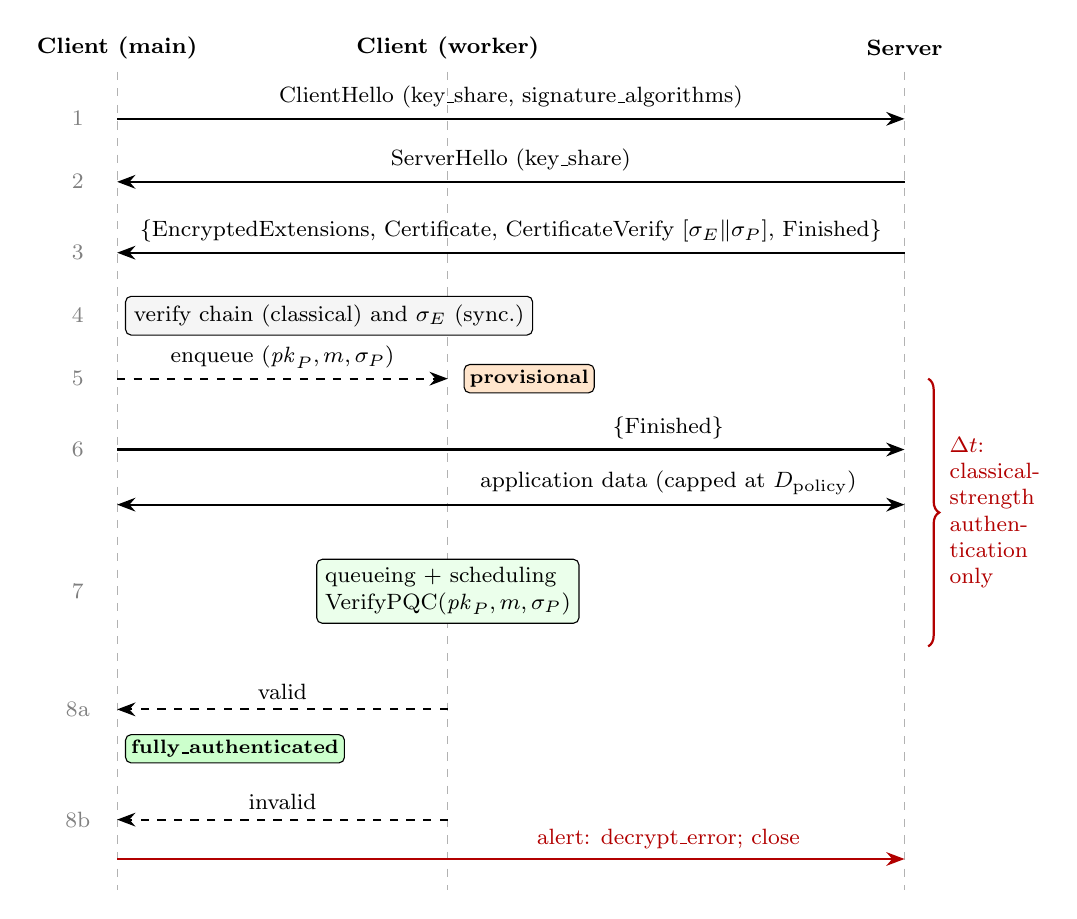
\begin{tikzpicture}[
  >=Stealth, font=\footnotesize,
  msg/.style={->, thick},
  note/.style={draw, rounded corners=2pt, align=left, inner sep=3pt,
               fill=gray!8},
  st/.style={draw, rounded corners=2pt, font=\scriptsize\bfseries,
             inner sep=2pt}
]
  \def\xa{0} \def\xb{4.2} \def\xc{10.0}
  \node[font=\footnotesize\bfseries] at (\xa,0.3) {Client (main)};
  \node[font=\footnotesize\bfseries] at (\xb,0.3) {Client (worker)};
  \node[font=\footnotesize\bfseries] at (\xc,0.3) {Server};
  \foreach \x in {\xa,\xb,\xc} \draw[gray!60, dashed] (\x,0) -- (\x,-10.4);
  % 1
  \node[gray] at (-0.5,-0.6) {1};
  \draw[msg] (\xa,-0.6) -- node[above]{ClientHello (key\_share, signature\_algorithms)} (\xc,-0.6);
  % 2
  \node[gray] at (-0.5,-1.4) {2};
  \draw[msg] (\xc,-1.4) -- node[above]{ServerHello (key\_share)} (\xa,-1.4);
  % 3
  \node[gray] at (-0.5,-2.3) {3};
  \draw[msg] (\xc,-2.3) -- node[above, align=center]{\{EncryptedExtensions, Certificate,
     CertificateVerify $[\sigma_E\|\sigma_P]$, Finished\}} (\xa,-2.3);
  % 4
  \node[gray] at (-0.5,-3.1) {4};
  \node[note, anchor=west] at (0.1,-3.1) {verify chain (classical) and $\sigma_E$ (sync.)};
  % 5
  \node[gray] at (-0.5,-3.9) {5};
  \draw[msg, dashed] (\xa,-3.9) -- node[above]{enqueue $(\mathit{pk}_P, m, \sigma_P)$} (\xb,-3.9);
  \node[st, fill=orange!20, anchor=west] at (\xb+0.2,-3.9) {\state{provisional}};
  % 6
  \node[gray] at (-0.5,-4.8) {6};
  \draw[msg] (\xa,-4.8) -- node[above, pos=0.7]{\{Finished\}} (\xc,-4.8);
  \draw[msg, <->] (\xa,-5.5) -- node[above, pos=0.7]{application data (capped at $D_\text{policy}$)} (\xc,-5.5);
  % 7
  \node[gray] at (-0.5,-6.6) {7};
  \node[note, anchor=center, fill=green!8] (pq) at (\xb,-6.6) {queueing + scheduling\\ $\mathrm{VerifyPQC}(\mathit{pk}_P, m, \sigma_P)$};
  % delta t brace
  \draw[decorate, decoration={brace, amplitude=4pt}, thick, red!70!black]
     (\xc+0.3,-3.9) -- node[right=4pt, align=left, text=red!70!black]
     {$\Delta t$:\\ classical-\\strength\\ authen-\\tication\\ only} (\xc+0.3,-7.3);
  % 8
  \node[gray] at (-0.5,-8.1) {8a};
  \draw[msg, dashed] (\xb,-8.1) -- node[above]{valid} (\xa,-8.1);
  \node[st, fill=green!20, anchor=west] at (0.1,-8.6) {\state{fully\_authenticated}};
  \node[gray] at (-0.5,-9.5) {8b};
  \draw[msg, dashed] (\xb,-9.5) -- node[above]{invalid} (\xa,-9.5);
  \draw[msg, red!70!black] (\xa,-10.0) -- node[above, pos=0.7]{alert: decrypt\_error; close} (\xc,-10.0);
\end{tikzpicture}
\caption{TLS~1.3 full handshake with DAPV on the client.  Messages in braces
  are encrypted under handshake traffic keys.  $\sigma_P$ is part of
  \texttt{CertificateVerify} and hence of the transcript authenticated by
  both \texttt{Finished} messages (step~3 onwards), so the deferred check in
  step~7 necessarily concerns the signature received in this handshake.
  No message is added or changed; steps 4--8 are local to the client.}
\label{fig:sequence}
\end{figure}

\subsection{Provisional-state semantics}
\label{sec:state_semantics}

\paragraph{Promotion does not re-key}  The transition from
\state{provisional} to \state{fully\_authenticated} changes only a local
state variable; no message is exchanged and the traffic keys are not
changed.  Re-keying is unnecessary because the keys depend only on the
(EC)DHE/KEM shared secret and the transcript, both fixed at step~6; the
PQ verification adds assurance about \emph{who} holds those keys, not about
the keys themselves.  If $\sigma_P$ verifies, the peer with whom the keys
were established during \Dt\ is the same peer that is now fully
authenticated, so data sent during \Dt\ is retroactively covered by the
full hybrid guarantee.  If it fails, that data may have been sent to an
impostor who defeated only the classical component; this is the exposure
bounded in Section~\ref{sec:leakage}.  A TLS \texttt{KeyUpdate} after
promotion is permissible but adds no authentication.

\paragraph{Data policy}  While \state{provisional}, the application may
send at most $D_\text{policy}$ bytes and should send only data it would be
willing to reveal to a classical-only authenticated peer
(Algorithm~\ref{alg:policy}).  Received data may be processed but should
not trigger irreversible actions.

\paragraph{Tickets, resumption and 0-RTT}  Because PSK resumption inherits
the authentication of the issuing session, a \texttt{NewSessionTicket}
received while \state{provisional} must be held and made usable only on
promotion, and discarded on failure.  Otherwise an attacker who passed only
the classical check could obtain a ticket whose resumptions---including
0-RTT early data---never undergo PQ verification.

\paragraph{Failure}  On PQ failure the client sends a fatal
\texttt{decrypt\_error} alert (the alert TLS~1.3 prescribes for a failed
\texttt{CertificateVerify}), closes the connection, marks the peer's
credential as failed for the lifetime of the process, and reports the
failure to the application.

\subsection{Transcript binding}
\label{sec:binding}

The server \texttt{Finished} MAC covers \texttt{CertificateVerify} and
therefore $\sigma_P$; the client verifies it before step~6.  An attacker
therefore cannot substitute $\sigma_P$ with a signature from another
session, or modify it in transit, without causing the server
\texttt{Finished} check to fail.  Binding guarantees \emph{which}
signature is verified later; it does not by itself guarantee that the
signature is \emph{valid}, which is precisely what step~7 checks.

\subsection{Algorithms}
\label{sec:algorithms}

Algorithm~\ref{alg:client} gives the client procedure.  $\mathrm{VerifyECDSA}$
and $\mathrm{VerifyPQC}$ denote the verification algorithms of ECDSA
P-256 and of the PQ scheme (ML-DSA.Verify of FIPS~204~\cite{FIPS204}
or FN-DSA verification~\cite{FIPS206Draft}), each applied to the
corresponding component public key $\mathit{pk}_E$, $\mathit{pk}_P$ from the
leaf certificate, the message $m$ of Section~\ref{sec:tls_auth} and the
corresponding signature component; each returns a Boolean.

\begin{algorithm}[t]
\caption{DAPV client processing of a hybrid \texttt{CertificateVerify}}
\label{alg:client}
\DontPrintSemicolon
\KwIn{Leaf keys $(\mathit{pk}_E, \mathit{pk}_P)$; message $m$; signature
  $\sigma_E \| \sigma_P$; session id $\mathit{sid}$}
\BlankLine
\If{\textbf{not} $\mathrm{VerifyECDSA}(\mathit{pk}_E, m, \sigma_E)$}{
  send alert \texttt{decrypt\_error}; abort \tcp*{no PQ work is scheduled}
}
$\mathrm{Submit}(\mathit{pk}_P, m, \sigma_P, \mathit{sid})$ to the worker
  pool (Algorithm~\ref{alg:server})\;
$\mathit{session}.\mathit{state} \leftarrow \state{provisional}$\;
verify server \texttt{Finished}; send client \texttt{Finished}; derive
  application traffic keys\;
\BlankLine
\SetKwProg{Proc}{on completion of job}{:}{}
\Proc{$(\mathit{sid}, \mathit{ok})$}{
  \eIf{$\mathit{ok}$}{
    $\mathit{session}(\mathit{sid}).\mathit{state} \leftarrow
      \state{fully\_authenticated}$; release held session tickets\;
  }{
    send alert \texttt{decrypt\_error}; close $\mathit{session}(\mathit{sid})$;
    discard held tickets\;
  }
}
\end{algorithm}

\paragraph{Dispatch order: after, not concurrently with, the classical check}  Two reasons.  First, dispatching only after $\sigma_E$
has verified ensures that a peer who cannot produce a valid classical
signature cannot cause any PQ work or occupy a worker; dispatching first
would let an unauthenticated attacker consume workers at the cost of a
single message, strengthening the flooding attack of
Section~\ref{sec:attacks}.  Second, the classical verification takes tens
of microseconds, so starting the PQ job earlier would shorten \Dt\ by at
most that amount.  Implementations that prefer to overlap the two can
dispatch first and cancel the job if $\sigma_E$ fails.

\begin{algorithm}[t]
\caption{Bounded verification worker pool (recommended design; the
  evaluated prototype uses one thread per job, Section~\ref{sec:impl})}
\label{alg:server}
\DontPrintSemicolon
\KwIn{Pool size $M$; queue capacity $Q$}
start $M$ worker threads, each executing:\;
\While{running}{
  $(\mathit{pk}_P, m, \sigma_P, \mathit{sid}) \leftarrow
    \mathrm{BlockingDequeue}()$\;
  $\mathit{ok} \leftarrow \mathrm{VerifyPQC}(\mathit{pk}_P, m, \sigma_P)$\;
  notify the owning connection of $(\mathit{sid}, \mathit{ok})$\;
}
\BlankLine
\SetKwProg{Fn}{function}{:}{}
\Fn{$\mathrm{Submit}(\mathit{pk}_P, m, \sigma_P, \mathit{sid})$}{
  \eIf{queue length $< Q$}{enqueue the job}{
    verify synchronously on the caller's thread \tcp*{back-pressure}
  }
}
\end{algorithm}

\begin{algorithm}[t]
\caption{Application-layer data policy}
\label{alg:policy}
\DontPrintSemicolon
\KwIn{Session state; bytes already sent while provisional $s$; payload
  size $d$; cap $D_\text{policy}$}
\eIf{$\mathit{state} = \state{provisional}$ \textbf{and}
     ($s + d > D_\text{policy}$ \textbf{or} payload is sensitive)}{
  buffer payload until \state{fully\_authenticated} (or drop on failure)\;
}{
  transmit payload; \lIf{$\mathit{state} = \state{provisional}$}{$s \leftarrow s + d$}
}
\end{algorithm}

\subsection{Design rationale: threads versus instruction-level parallelism}
\label{sec:why_threads}

A natural question is why DAPV uses a separate thread when PQ verification
is already fast and vector instructions (AVX2, AVX-512) accelerate it
further.  The two techniques are complementary rather than alternatives.
SIMD reduces the \emph{duration} of one verification and is already used
by our prototype (liboqs AVX2 code paths).  Thread-level deferral changes
\emph{where} the remaining duration is spent: off the handshake critical
path.  For a single AVX2 ML-DSA-44 verification the remaining duration is
about 0.1\ms, and deferring it cannot save more than that; we confirm in
Section~\ref{sec:res_where} that the latency gain we measure is \emph{not}
explained by this cost.

Deferral becomes worthwhile when the synchronous PQ work on the critical
path is large, which happens when (i) the chain contains several
PQ-signed certificates, possibly with PQ-signed certificate-transparency
timestamps, so that a handshake needs several PQ verifications; (ii) a
slower scheme such as SLH-DSA is used; (iii) the client lacks vector units
(microcontrollers, low-end ARM cores); or (iv) the credential combines more
than two algorithms (e.g., ECDSA\,+\,ML-DSA\,+\,SLH-DSA).  Cases (i) and
(iv) consist of \emph{independent} verifications, which SIMD cannot
parallelise with one another but a worker pool can, one per core.
Algorithm~\ref{alg:client} generalises directly: all PQ components are
submitted as separate jobs and the session is promoted when all have
succeeded.  We have not evaluated these cases; they are the most promising
direction for follow-up measurements
\authorinput{if you add experiments with 2--3-certificate chains or
three-algorithm hybrids, report them here}.

\subsection{Analytical model}
\label{sec:analytical}

Let $k$ be the number of round trips of the handshake (one for a TLS~1.3
full handshake as seen by the client) and $L_0$ the RTT-independent
processing time.  Then
\begin{equation}
  L = L_0 + (k + \delta k)\,\mathrm{RTT},
  \label{eq:latency}
\end{equation}
where $\delta k \ge 0$ counts additional round trips, which occur when the
server's first flight exceeds the sender's congestion window (initially
about ten segments~\cite{RFC6928}), \emph{not} merely when a message spans
several segments: segments within the window are sent back to back.
DAPV removes the synchronous PQ-path time $T_\text{PQ}$ from $L_0$ and
leaves $\delta k$ unchanged:
\begin{equation}
  L_\text{DAPV} = (L_0 - T_\text{PQ}) + (k + \delta k)\,\mathrm{RTT}.
  \label{eq:dapv}
\end{equation}
Consequently the saving is an RTT-independent offset, $T_\text{PQ}$, and
the curves of synchronous and DAPV latency against RTT have equal slope.
For the single-certificate configuration used in our experiments the
server flight is approximately 7~KB (two ML-DSA-44 signatures, one
ML-DSA-44 public key, the classical components and certificate overhead),
below the initial window, so we expect $\delta k = 0$; our measurements
(Section~\ref{sec:res_latency}) agree.

%% ============================================================
\section{Implementation and Experimental Setup}
\label{sec:setup}

\subsection{Implementation}
\label{sec:impl}

The prototype is built on OpenSSL~3.2, liboqs \authorinput{version} and the
OQS provider \authorinput{version}~\cite{OQS2017}.  Hybrid certificates
carry the concatenation of the P-256 and PQ public keys; signatures are
encoded as $\mathrm{len}(\sigma_E)\|\sigma_E\|\sigma_P$.  We modified the
provider's hybrid signature-verification routine
(\texttt{oqs\_sig\_verify}) so that, when invoked for the server's
\texttt{CertificateVerify}, it verifies the classical component, copies
$(\mathit{pk}_P, m, \sigma_P)$ into a job, dispatches it with
\texttt{CreateThread} (Windows) or \texttt{pthread\_create} (Linux), and
returns success to OpenSSL so that the handshake proceeds.  A per-connection
state object, reachable through \texttt{SSL\_get\_ex\_data}, records the
state and receives the job result; on failure the main thread sends the
alert at its next I/O operation \authorinput{confirm mechanism, e.g.,
polled flag or wake-up via socket pair}.  The prototype creates one thread
per job; the bounded pool of Algorithm~\ref{alg:server} and the ticket
handling of Section~\ref{sec:state_semantics} are \authorinput{implemented /
not implemented in the prototype---state which}.

\subsection{Code and data availability}
\label{sec:availability}

The source code of the modified provider, the load generator, the
measurement scripts and the raw measurements are available at
\authorinput{public repository URL and archived DOI (e.g., Zenodo)}.

\subsection{Hardware and operating systems}

Two x86-64 testbeds were used: an Intel Core i7-11800H (8~cores,
2.3~GHz, 32~GB RAM) running Windows~11 Pro, and an Intel Xeon Silver~4310
(12~cores, 2.1~GHz, 64~GB RAM) running Ubuntu~22.04 LTS; AVX2 was enabled
on both.  Compilers were Visual Studio~2022 and GCC~11.3.  On each testbed,
the TLS client (load generator) and server ran on the same host
\authorinput{confirm; state CPU pinning of client and server processes, if
any}.  Results in Section~\ref{sec:results} are from the
\authorinput{Windows / Linux} testbed unless stated otherwise.

\subsection{Cryptographic configuration}
\label{sec:crypto_config}

Server authentication used five configurations: ECDSA P-256 (classical
baseline); ML-DSA-44 and FN-DSA-512 alone (synchronous PQ-only baselines);
and the hybrids P-256\,+\,ML-DSA-44 and P-256\,+\,FN-DSA-512, each measured
with synchronous verification and with DAPV.  Key exchange used the group
\authorinput{state the group actually negotiated, e.g., X25519 or
X25519MLKEM768} in \emph{all} configurations, so that differences between
configurations are attributable to authentication alone.
\authorinput{If the group was X25519: add ``Using X25519MLKEM768 instead
would add 1216 and 1120 bytes to ClientHello and ServerHello respectively
and about 0.1\,ms of computation to both sides, but would not interact
with signature verification; the results therefore transfer to a full PQ
configuration except for these additive terms.'' Better: re-run the hybrid
configurations with X25519MLKEM768.}

\subsection{Network emulation}

Delay was added with Clumsy~0.3 (Windows) and \texttt{tc netem} (Linux) to
obtain RTTs of 0, 20, 50, 100 and 150\ms, without packet loss.  On Linux
the qdisc was attached to \authorinput{interface---if the loopback
interface, state how delay was split between directions}.

\subsection{Metrics and procedure}

\begin{enumerate}[leftmargin=*,noitemsep]
\item \textbf{Handshake latency}: at the client, from sending
  \texttt{ClientHello} to the point at which the client may send
  application data (after sending its \texttt{Finished}), i.e., the
  latency seen by the application.
\item \textbf{Completed-handshake rate}: handshakes completed per second by
  a closed-loop load generator with 100, 500 or 1000 concurrent clients,
  each opening a new connection as soon as its previous handshake
  completes \authorinput{confirm tool and closed-loop behaviour; confirm
  sessions are not resumed}.  Because client and server share a host, this
  is a system-level rate, not a server-only capacity.
\item \textbf{Peak CPU utilisation} of the host during a run.
\item \textbf{\Dt}: from job submission (step~5) to completion of PQ
  verification (step~7), decomposed into the verification call alone, timed
  inside the worker, and the remainder (thread creation, queueing and
  scheduling).
\end{enumerate}
Each configuration was measured in 30 independent runs
\authorinput{state how many handshakes per run}.  With the observed
standard deviations of latency and throughput (below 4\% of the mean), 30
runs give a 95\% confidence-interval half-width of about 1.5\% of the mean,
which is an order of magnitude smaller than the differences we report.
\Dt\ is considerably more dispersed (Table~\ref{tab:delta_t}); its tail
percentiles are reported as descriptive statistics of the pooled samples.

%% ============================================================
\section{Results}
\label{sec:results}

\subsection{Handshake latency}
\label{sec:res_latency}

\begin{figure}[t]
  \centering
  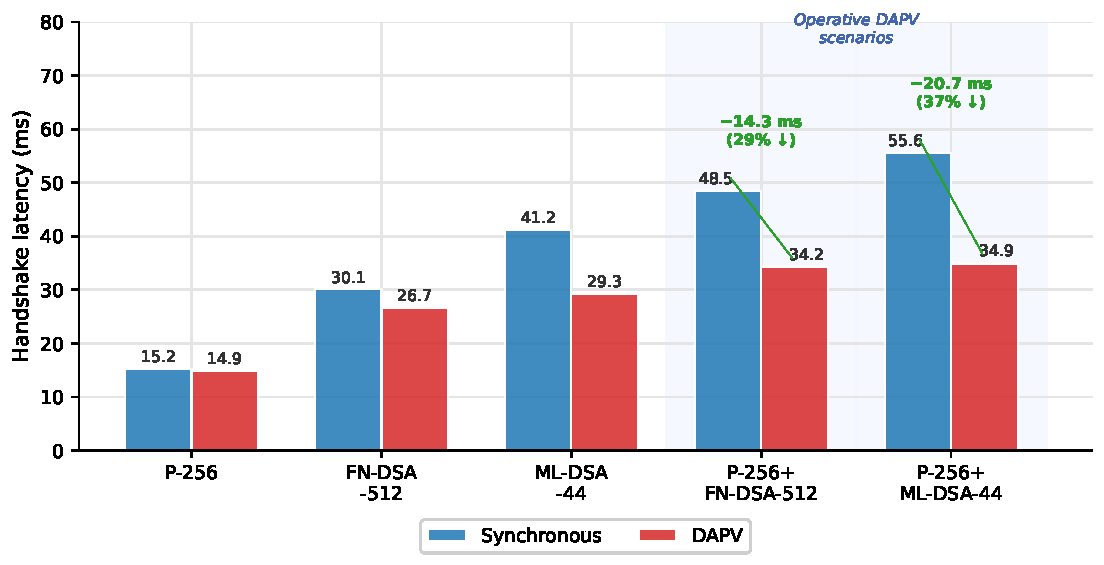
\includegraphics[width=0.8\columnwidth]{fig01_latency_bar_0ms.pdf}
  \caption{Handshake latency at 0\ms\ added RTT, synchronous (blue) versus
    DAPV (red).  For standalone PQ configurations, the DAPV bars quantify
    thread overhead only; they are not operative deployments.}
  \label{fig:latency_bar}
\end{figure}

\begin{figure}[t]
  \centering
  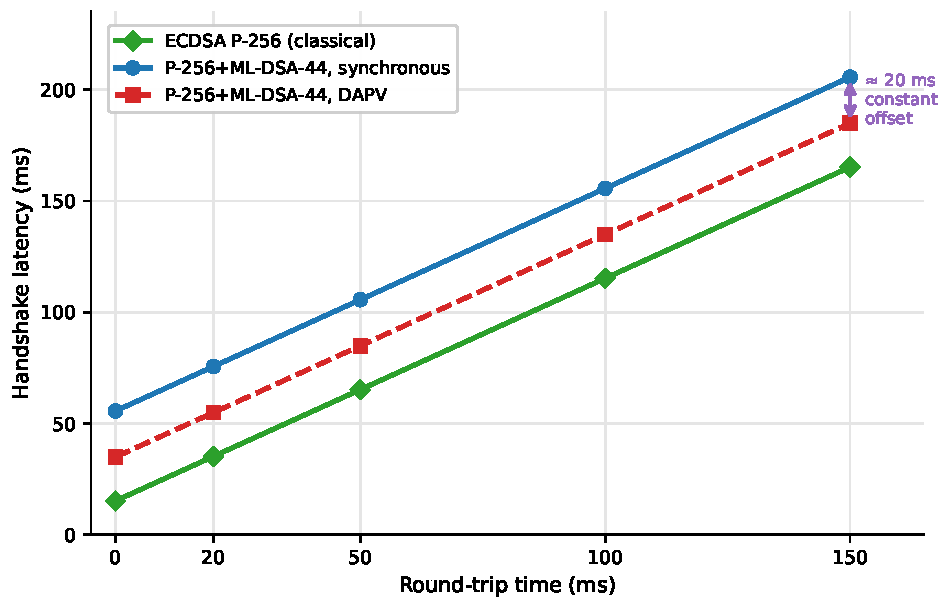
\includegraphics[width=0.8\columnwidth]{fig02_latency_vs_rtt.pdf}
  \caption{Handshake latency versus RTT for P-256\,+\,ML-DSA-44.  The three
    curves have the same slope; DAPV is offset by $\approx$20\ms\ from
    synchronous hybrid at every RTT.
    \authorinput{Confirm that the points at RTT = 20, 50 and 100\,ms are
    measured. If they were interpolated, remove those markers.}}
  \label{fig:latency_rtt}
\end{figure}

\emph{Takeaway: DAPV lowers latency by an RTT-independent offset; it does not
change the slope.}  At 0\ms\ RTT (Figure~\ref{fig:latency_bar}), DAPV
lowers latency from 48.5 to 34.2\ms\ for P-256\,+\,FN-DSA-512 ($-29\%$)
and from 55.6 to 34.9\ms\ for P-256\,+\,ML-DSA-44 ($-37\%$).  Against RTT
(Figure~\ref{fig:latency_rtt}) the classical, synchronous-hybrid and DAPV
curves all have a slope of 1.0\,ms per ms of RTT.  For P-256\,+\,ML-DSA-44
the DAPV saving is 20.7\ms\ at 0\ms\ RTT and 21.0\ms\ at 150\ms, i.e.,
RTT-independent to within measurement precision.  For P-256\,+\,FN-DSA-512
the saving is 14.3\ms\ at 0\ms\ and 20.0\ms\ at 150\ms\ RTT
\authorinput{this growth is not predicted by Equation~\eqref{eq:dapv};
please check both values against the raw data and explain or correct}.
Equal slopes mean $\delta k = 0$ in our configuration, as predicted in
Section~\ref{sec:analytical}.  The relative saving therefore falls with
RTT---from 37\% to 10\% for P-256\,+\,ML-DSA-44---because the absolute
saving is fixed while the RTT term grows.

\subsection{Where does the latency saving come from?}
\label{sec:res_where}

\emph{Takeaway: the saving is two orders of magnitude larger than the cost
of PQ arithmetic.}  Timed in isolation, a PQ verification takes
0.08--0.14\ms\ (Table~\ref{tab:delta_t}), yet DAPV saves 14--21\ms.
The saving must therefore come from other work on the synchronous
verification path of the prototype, which in the synchronous build runs
inline on the handshake thread and in the DAPV build runs on the worker.
Candidates are per-call provider dispatch and key decoding, memory
allocation, and waiting that is quantised by the operating-system timer:
the default timer period on Windows is 15.6\ms, close to both the saving
and the scheduling component of \Dt.
\authorinput{Profile the synchronous verification path (e.g., perf,
VTune or ETW) and report the breakdown here. Report the Linux-testbed
saving and \Dt; if the Windows timer resolution is the cause, the Linux
values should be much smaller.}

This finding has a direct consequence that we state plainly: for a single
hybrid signature on a desktop-class CPU, most of the benefit we measure
could also be obtained by optimising the synchronous path.  The
contribution of deferral itself is bounded by the synchronous PQ work that
remains on the critical path, which is small in our configuration and
larger in the cases listed in Section~\ref{sec:why_threads}.

\subsection{Completed-handshake rate}
\label{sec:res_throughput}

\begin{figure}[t]
  \centering
  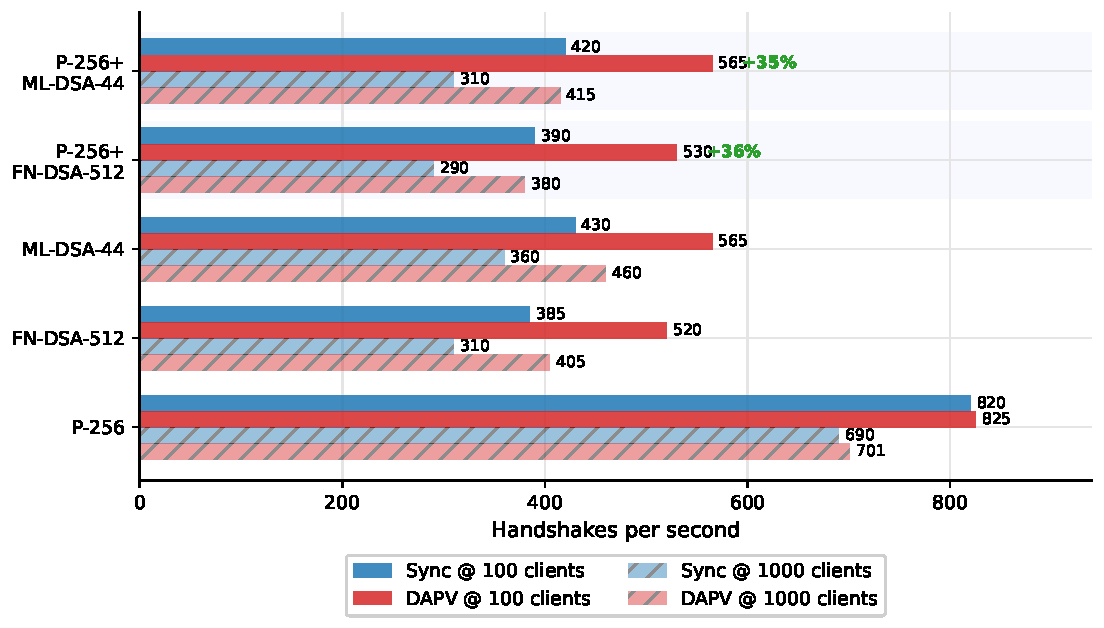
\includegraphics[width=0.8\columnwidth]{fig04_throughput_bar.pdf}
  \caption{Completed handshakes per second with 100 (solid) and 1000
    (hatched) concurrent clients; client and server on the same host.}
  \label{fig:throughput_bar}
\end{figure}

\begin{figure}[t]
  \centering
  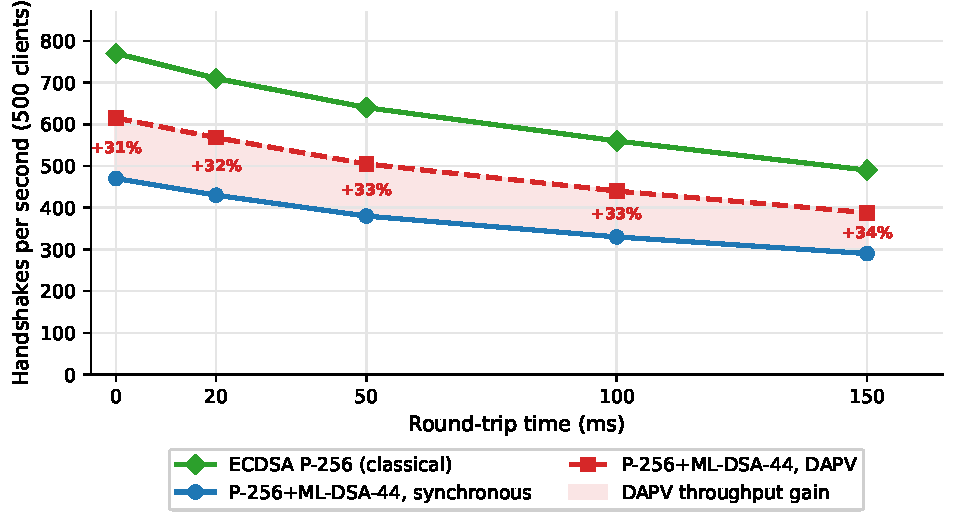
\includegraphics[width=0.8\columnwidth]{fig05_throughput_vs_rtt.pdf}
  \caption{Completed handshakes per second versus RTT at 500 concurrent
    clients, P-256\,+\,ML-DSA-44.}
  \label{fig:throughput_rtt}
\end{figure}

\emph{Takeaway: with client and server on one host, DAPV raises the
completed-handshake rate by 31--36\%, consistently across concurrency and
RTT.}  Hybrid authentication lowers the rate from 820 to 390--420
handshakes/s at 100 clients and from 690 to 290--310 at 1000 clients (55--58\%), relative to classical ECDSA (Figure~\ref{fig:throughput_bar}).  DAPV
raises it by 35--36\% at 100 clients, 31\% at 500 clients
(Table~\ref{tab:summary}) and 31--34\% at 1000 clients.  Across RTT at 500
clients (Figure~\ref{fig:throughput_rtt}) the gain for
P-256\,+\,ML-DSA-44 stays between 31\% and 34\%.

Because DAPV changes only the client, it cannot reduce the server's
cryptographic work.  Two mechanisms can raise the measured rate: the
client-side load generator, which competes with the server for the same
cores, spends less time blocked per handshake; and each connection holds
server resources for a shorter time because the client \texttt{Finished}
arrives earlier.  Our single-host setup cannot separate them, and the first
mechanism would not appear with clients on separate machines.  The rate
gain must therefore be read as a property of the combined client--server
system, not as a server capacity gain.
\authorinput{Re-run with load generator and server on separate hosts
(or at least pinned to disjoint cores) and report server-only throughput.}

\subsection{CPU utilisation}
\label{sec:res_cpu}

\emph{Takeaway: DAPV redistributes but does not reduce CPU work.}  Peak host
CPU utilisation is 35\% for classical ECDSA and 79--85\% for the hybrid
configurations, with and without DAPV (Table~\ref{tab:summary}); the same
operations execute in both cases, but under DAPV the PQ verification runs
on worker threads concurrently with other connections.

\subsection{Provisional window \Dt}
\label{sec:res_delta_t}

\begin{table}[t]
\centering
\caption{Decomposition of \Dt\ on idle hardware (30 runs; ms).  ``Crypto''
  is the verification call timed inside the worker; ``Scheduling'' is the
  remainder (thread creation, queueing, wake-up).}
\label{tab:delta_t}
\small
\begin{tabular}{lrrrr}
\toprule
\textbf{Configuration} & \textbf{Crypto} & \textbf{Scheduling} &
\textbf{Total \Dt\ (mean)} & \textbf{95\% CI of mean} \\
\midrule
P-256\,+\,FN-DSA-512  & 0.14 & 18.76 & 18.9 & [16.7,\;21.1] \\
P-256\,+\,ML-DSA-44   & 0.10 & 21.10 & 21.2 & [18.6,\;23.8] \\
\bottomrule
\end{tabular}
\end{table}

\begin{figure}[t]
  \centering
  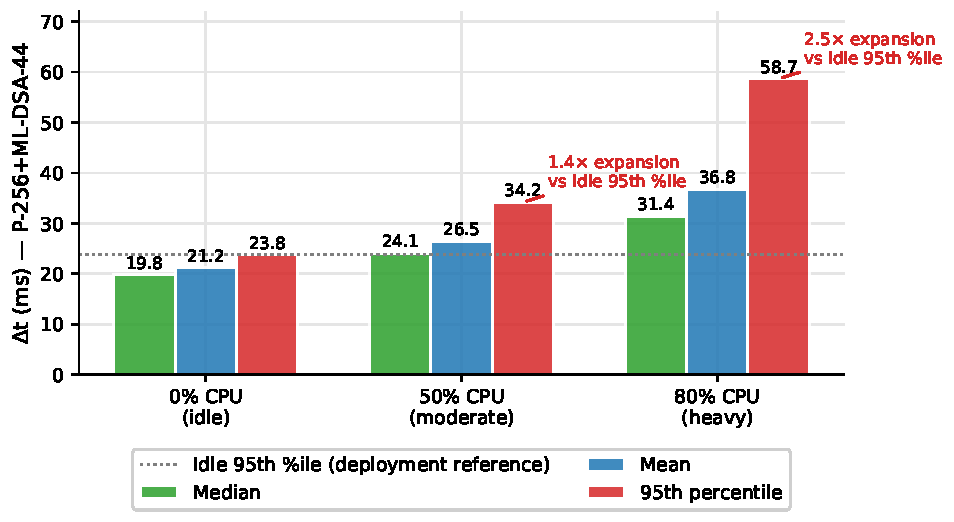
\includegraphics[width=0.8\columnwidth]{fig09_delta_t_vs_cpu_load.pdf}
  \caption{\Dt\ for P-256\,+\,ML-DSA-44 under 0\%, 50\% and 80\% background
    CPU load: median, mean and 95th percentile.}
  \label{fig:deltat_load}
\end{figure}

\emph{Takeaway: \Dt\ is set by scheduling, not cryptography, and grows
under load.}  Table~\ref{tab:delta_t} shows that the verification itself is
under 1\% of \Dt; the rest is scheduling.  Under background CPU load
(Figure~\ref{fig:deltat_load}), the 95th percentile of \Dt\ grows from
23.8\ms\ (idle) to 34.2\ms\ at 50\% and 58.7\ms\ at 80\% load, i.e.,
$2.5\times$ the idle 95th percentile.  Any data cap must therefore be
calibrated against loaded, not idle, \Dt.  A bounded pool with pre-started
workers (Algorithm~\ref{alg:server}) removes thread creation from \Dt\ and
should bring it close to the queueing plus verification time; we have not
measured such an implementation, and the value it would achieve is a
projection, not a result \authorinput{if you implement and measure the
pool, report the measured \Dt\ here}.

\subsection{Summary}
\label{sec:res_summary}

\begin{table}[t]
\centering
\caption{Summary of measured results.  Rate and CPU at 500 concurrent
  clients and 0\ms\ RTT; \Dt\ is the idle mean.  Only measured values are
  shown.}
\label{tab:summary}
\small
\setlength{\tabcolsep}{5pt}
\begin{tabular}{lrrrrr}
\toprule
\textbf{Configuration} & \textbf{Latency 0\ms} & \textbf{Latency 150\ms} &
  \textbf{Rate} & \textbf{Peak CPU} & \textbf{\Dt} \\
& (ms) & (ms) & (hs/s) & (\%) & (ms) \\
\midrule
ECDSA P-256                         & 15.2 & 165 & 770 & 35 & --- \\
FN-DSA-512, synchronous             & 30.1 & 180 & 380 & 76 & --- \\
ML-DSA-44, synchronous              & 41.2 & 191 & 390 & 82 & --- \\
P-256\,+\,FN-DSA-512, synchronous   & 48.5 & 199 & 440 & 85 & --- \\
P-256\,+\,FN-DSA-512, DAPV          & 34.2 & 179 & 575 (+31\%) & 85 & 18.9 \\
P-256\,+\,ML-DSA-44, synchronous    & 55.6 & 206 & 470 & 79 & --- \\
P-256\,+\,ML-DSA-44, DAPV           & 34.9 & 185 & 615 (+31\%) & 79 & 21.2 \\
\bottomrule
\end{tabular}
\end{table}

Table~\ref{tab:summary} collects the measured values.  Relative to
classical ECDSA at 150\ms\ RTT, synchronous P-256\,+\,ML-DSA-44 adds 25\%
latency and DAPV 12\%; at 500 clients the completed-handshake rate is 39\%
below classical for the synchronous hybrid and 20\% below with DAPV.

\subsection{Threats to validity}
\label{sec:threats}

\begin{itemize}[leftmargin=*]
\item \textbf{Co-location.}  Client and server share a host, so they compete
  for CPU and the rate measurements include client-side effects
  (Section~\ref{sec:res_throughput}).  Traffic between them does not cross
  a physical network interface.
\item \textbf{Emulated network.}  On the loopback interface, the MTU is
  64~KB and segmentation offload is typical, so segment counts and
  congestion-window behaviour differ from those on a real path; delay-only
  emulation without loss or bandwidth limits does not exercise loss
  recovery.  Our conclusions about $\delta k$ apply to the emulated setting;
  in particular, we do not claim to have measured the effect of MTU-sized
  segmentation.
\item \textbf{Certificate chain.}  A single-certificate chain understates
  the size and the number of verifications of real deployments, which
  typically send a leaf and one intermediate (and embed SCTs).  Longer
  chains would increase both the size cost (possibly making $\delta k > 0$)
  and the PQ work that DAPV can defer.
\item \textbf{Timer resolution.}  Several reported durations are of the same
  order as the Windows timer period (Section~\ref{sec:res_where}).
\item \textbf{Prototype concurrency model.}  One thread per job; the
  recommended bounded pool was not evaluated.
\end{itemize}
\authorinput{Where you have new data from separate hosts, real NICs or
longer chains, report it and shorten this list accordingly.}

%% ============================================================
\section{Security Analysis}
\label{sec:security}

The analysis below is a risk characterisation, not a proof.  A formal
analysis of the provisional state---e.g., in Tamarin, extending
existing TLS~1.3 models~\cite{Cremers2017}---is future work.

\subsection{Threat model}

The network adversary controls the channel (Dolev--Yao).  We distinguish
(i) a \emph{classical} adversary, who cannot forge ECDSA or PQ signatures
but might hold a fraudulently issued classical credential or exploit a flaw
in the classical component, and (ii) a \emph{CRQC} adversary, who can forge
ECDSA.  Against (i), DAPV provides the same final guarantee as synchronous
hybrid verification, but data sent during \Dt\ reaches a peer
authenticated only classically.  Against (ii), the provisional state offers
no protection: DAPV is appropriate only while CRQCs capable of real-time
forgery are not a practical threat, and deployments must reassess it as
that changes.

\subsection{Leakage bound}
\label{sec:leakage}

The data the client can send before a failed PQ check tears down the
connection is bounded by the link rate and by the TCP congestion window:
\begin{equation}
  L_\text{max} = \min\!\left(\frac{B\,\Dt}{8},\; W(\Dt)\right),
  \label{eq:leakage}
\end{equation}
where $B$ is the bottleneck bandwidth in bit/s and $W(\Dt)$ is the amount
the client's congestion controller allows in flight during \Dt\ on a new
connection (about 14.6~KB per RTT at the initial window~\cite{RFC6928}).
When $\Dt < \mathrm{RTT}$, $W(\Dt)$ is at most one initial window, so the
exposure is limited to about 14.6~KB irrespective of link speed; the
bandwidth term dominates only on low-RTT paths.  Table~\ref{tab:leakage}
gives the bandwidth term; the application cap $D_\text{policy}$ bounds both.

\begin{table}[t]
\centering
\caption{Bandwidth term $B\,\Dt/8$ of Equation~\eqref{eq:leakage} for
  measured \Dt\ values (decimal units).  The last column is a hypothetical
  \Dt\ of 1\ms, not a measured value.}
\label{tab:leakage}
\small
\begin{tabular}{lrrrr}
\toprule
& \multicolumn{3}{c}{\textbf{Measured \Dt}} & \textbf{Hypothetical} \\
\cmidrule(lr){2-4}
\textbf{Link rate} & 18.9\ms\ & 21.2\ms\ & 58.7\ms\ (p95, 80\% load) & 1\ms \\
\midrule
1 Mbit/s   & 2.4 kB   & 2.7 kB   & 7.3 kB   & 125 B   \\
100 Mbit/s & 236 kB   & 265 kB   & 734 kB   & 12.5 kB \\
1 Gbit/s   & 2.4 MB   & 2.7 MB   & 7.3 MB   & 125 kB  \\
10 Gbit/s  & 24 MB    & 27 MB    & 73 MB    & 1.25 MB \\
\bottomrule
\end{tabular}
\end{table}

\paragraph{Choice of $D_\text{policy}$}  The cap is a policy parameter,
not a quantity our measurements determine.  Its correct value is the
amount of data the application is willing to reveal to a peer that has
passed only the classical check, which depends on the content, not on
\Dt.  What \Dt\ determines is how often the cap is reached and hence how
often data must be buffered.  As a heuristic default we suggest 8~KB: it
is below one initial congestion window, so on WAN paths the cap rather than
TCP is the binding limit; it is roughly the bandwidth term at 1~Mbit/s
for the loaded 95th-percentile \Dt\ (7.3~kB), so on slow links the cap is
rarely reached; and it accommodates typical request headers and small
requests.  Applications should lower it, or set it to zero, for any
content they consider sensitive.

\subsection{Attack vectors and mitigations}
\label{sec:attacks}

\paragraph{Impersonation with a valid classical credential}  An adversary
holding a fraudulently obtained classical key for the server passes step~4
and receives up to $L_\text{max}$ bytes before step~8 terminates the
session.  Mitigation: $D_\text{policy}$ and the restriction to
non-sensitive content.

\paragraph{Component stripping}  Replacing $\sigma_P$ with an invalid
value causes the server \texttt{Finished} check to fail (transcript
binding); presenting a classical-only credential is rejected because the
client requires the hybrid algorithm.  Either way no session is promoted.

\paragraph{Replay}  A \texttt{CertificateVerify} from another session does
not verify against this session's transcript hash, which includes both
parties' fresh key shares.

\paragraph{Ticket inheritance}  Addressed by holding tickets until
promotion (Section~\ref{sec:state_semantics}).

\paragraph{Worker exhaustion (DAPV-specific)}  In mutual-TLS or other
settings where the verifier accepts many handshakes---e.g., a server
verifying hybrid client certificates with DAPV---an adversary can send a
valid $\sigma_E$ with an invalid $\sigma_P$ on many connections, each
occupying a worker until its job fails.  With one thread per job this
exhausts memory and threads.  Mitigations: a bounded pool with bounded
queue and synchronous fall-back (Algorithm~\ref{alg:server}), which
degrades DAPV to synchronous verification under attack instead of failing;
and per-source rate limiting.  Dispatching only after $\sigma_E$ succeeds
(Algorithm~\ref{alg:client}) means the attack requires a valid classical
signature per connection.

\subsection{Application-layer interface}
\label{sec:api}

Enforcing $D_\text{policy}$ requires the TLS library to expose the state.
We propose the following minimal OpenSSL-style interface
\authorinput{state whether this interface is implemented in the prototype
or is a proposal}:
\begin{verbatim}
#define SSL_DAPV_STATE_NONE        0   /* not a DAPV session        */
#define SSL_DAPV_STATE_PROVISIONAL 1   /* sigma_E ok, sigma_P pending */
#define SSL_DAPV_STATE_FULL_AUTH   2   /* sigma_E and sigma_P ok     */
#define SSL_DAPV_STATE_PQC_FAILED  3   /* sigma_P failed; closed    */

int  SSL_get_dapv_state(const SSL *ssl);
void SSL_CTX_set_dapv_callback(SSL_CTX *ctx,
         void (*cb)(SSL *ssl, int new_state, void *arg), void *arg);
\end{verbatim}
The callback is invoked on each state change, allowing an application to
release buffered data on promotion and to abort pending work on failure;
\texttt{SSL\_write} can enforce $D_\text{policy}$ by returning a
retry-later indication while the session is provisional and the cap is
reached.

%% ============================================================
\section{Deployment Considerations}
\label{sec:deployment}

\paragraph{Where DAPV fits}  DAPV suits clients that (i) can tolerate a
bounded interval of classical-strength authentication for their first
bytes, and (ii) perform enough synchronous PQ work per handshake for its
removal to matter: long PQ chains, multi-algorithm credentials, SLH-DSA,
or devices without vector units.  Browsers fetching public content, API
clients sending idempotent requests, and edge proxies are examples.
Clients that immediately send credentials, payment data or personal data
should verify synchronously or set $D_\text{policy} = 0$ for such
requests.

\paragraph{Operational requirements}  A bounded worker pool; exposure of
the provisional state to applications; monitoring of \Dt\ (mean and
95th percentile), PQ failure rate and provisional-session count;
calibration of any cap against \Dt\ under production load; and the ticket
rules of Section~\ref{sec:state_semantics}.

\paragraph{Device classes}  On devices without vector units the
verification itself becomes the dominant term of \Dt, increasing both the
benefit of deferral and the exposure window.  We have not measured such
devices; published microcontroller benchmarks~\cite{pqm4} suggest
verification times of milliseconds rather than tenths of a millisecond,
and a deployment there should re-measure \Dt\ before choosing
$D_\text{policy}$.

\paragraph{Standardisation}  Because DAPV changes no messages, it needs no
TLS extension to interoperate.  What would benefit from standardisation is
guidance on the provisional semantics---ticket handling, permitted data and
alerting---for implementations that choose to defer, analogous to the
guidance that accompanied TLS False Start~\cite{RFC7918}.

%% ============================================================
\section{Comparison with Prior Work}
\label{sec:comparison}

Table~\ref{tab:priorwork} contrasts DAPV with prior work by target and
method.  Numerical comparison across studies is not meaningful because
testbeds, chains and network conditions differ.

\begin{table}[t]
\centering
\caption{Positioning relative to prior work.}
\label{tab:priorwork}
\small
\begin{tabular}{p{3.6cm}p{3.6cm}p{6.2cm}}
\toprule
\textbf{Work} & \textbf{Cost addressed} & \textbf{Approach} \\
\midrule
\cite{Paquin2020,Sikeridis2020a,Sikeridis2020b,Sosnowski2023,Montenegro2026}
  & size and computation & measurement; no mitigation \\
\cite{KampanakisKallitsis2022,Sikeridis2022ICA,Paul2022}
  & size (chain) & omit or change certificates in the chain \\
\cite{Schwabe2020KEMTLS,Schwabe2021,WiggersIETF2024}
  & size (handshake signature) & KEM-based implicit authentication \\
\cite{Hu2019QTLS}
  & computation (throughput) & asynchronous offload; connection waits for result \\
This work & computation (latency) & defer PQ verification past handshake completion
  under a provisional state \\
\bottomrule
\end{tabular}
\end{table}

%% ============================================================
\section{Conclusion}
\label{sec:conclusion}

We studied deferring the PQ component of hybrid TLS~1.3 server
authentication past handshake completion.  DAPV requires no protocol
change and is defined by the semantics of a provisional client state:
classical authentication at completion, promotion on PQ success, teardown
on failure, a data cap, and tickets withheld until promotion.  In our
prototype and single-host testbed, it lowers handshake latency by an
RTT-independent 14--21\ms\ and raises the completed-handshake rate by
31--36\%.  Our decomposition shows that these gains exceed the cost of PQ
arithmetic by two orders of magnitude, so for a single signature on a
modern desktop CPU they reflect the cost of the prototype's synchronous
path rather than an intrinsic benefit of deferral.  Deferral is most
relevant where synchronous PQ work is genuinely large: multi-certificate
chains, multi-algorithm credentials, slow schemes and constrained
devices.  The exposure it creates is bounded by the data cap and, on WAN
paths, by the TCP initial window.

\subsection*{Future work}
\begin{enumerate}[noitemsep]
\item Measurements with separate client and server hosts over real network
  interfaces, 2--3-certificate chains and X25519MLKEM768 key exchange.
\item Multi-algorithm hybrids and SLH-DSA, where several independent
  verifications can be parallelised across workers.
\item A bounded-pool implementation and its measured \Dt.
\item A formal (e.g., Tamarin) model of the provisional state.
\item Server-side deferral for hybrid client certificates in mutual TLS.
\item Evaluation on ARM and microcontroller platforms.
\end{enumerate}

\section*{Acknowledgements}
The authors thank the Open Quantum Safe project and the OpenSSL community
for the open-source infrastructure used in this work.

\section*{Declaration of Competing Interest}
The authors declare no competing financial interests or personal
relationships that could have influenced the work reported in this paper.

\bibliographystyle{elsarticle-num}
\bibliography{references}

\end{document}
